%!TEX root = ../../Heun_Dale_Haney_A_dynamic_approach_to_input_output_modeling.tex
%%%%%%%%%%%%%%%%%%%%% chapter.tex %%%%%%%%%%%%%%%%%%%%%%%%%%%%%%%%%
%
% sample chapter
%
% Use this file as a template for your own input.
%
%%%%%%%%%%%%%%%%%%%%%%%% Springer-Verlag %%%%%%%%%%%%%%%%%%%%%%%%%%
%\motto{Use the template \emph{chapter.tex} to style the various elements of your chapter content.}
\motto{Where there is no reliable accounting 
and therefore no competent knowledge
of the economic and ecological effects of our lives,
we cannot live lives that are economically
and ecologically responsible. 
It is futile to plead and protest and lobby 
in favor of public ecological responsibility while, 
in virtually every act of our private lives, 
we endorse and support an economic system 
that is by intention, 
and perhaps by necessity, 
ecologically irresponsible.~\emph{\cite[p.~26]{Berry1998}}

\hfill---\emph{Wendell Berry}}


\chapter{Introduction}
% use \chaptermark{}
% to alter or adjust the chapter heading in the running head
\chaptermark{Introduction}
% Always give a unique label
\label{chap:intro}

\abstract*{[NEED TO ADD ABSTRACT HERE]}

%% \abstract{Each chapter should be preceded by an abstract (10--15 lines long) that summarizes the content. The abstract will appear \textit{online} at \url{www.SpringerLink.com} and be available with unrestricted access. This allows unregistered users to read the abstract as a teaser for the complete chapter. As a general rule the abstracts will not appear in the printed version of your book unless it is the style of your particular book or that of the series to which your book belongs.\newline\indent
%% Please use the 'starred' version of the new Springer \texttt{abstract} command for typesetting the text of the online abstracts (cf. source file of this chapter template \texttt{abstract}) and include them with the source files of your manuscript. Use the plain \texttt{abstract} command if the abstract is also to appear in the printed version of the book.}

%% Use the template \emph{chapter.tex} together with the Springer document class SVMono (monograph-type books) or SVMult (edited books) to style the various elements of your chapter content in the Springer layout.

%DISCUSSION POINTS
%\begin{itemize}
%	% \item{Is `society' the best word – `final consumption?'}
%	%	\item{Do we use energy circuit language?}
%	% \item{For economists, capital is only in the productive sector, 
%	%$\dot{K}_{i1}$ flows would be `consumer durables'}
%	\item{Housing is `residential capital'}
%\end{itemize}

This book is primarily about accounting and change.
It is borne out of a belief that our economies are in constant flux;
changing dynamically in the short-term with human behavior
and evolving over longer time frames 
in response to technological change and
external pressures.
Real-world systems, including economies, are messy and chaotic.
They do not march orderly from one state to the next.

% This is also a book about models and metaphors.
% The real world influences the mental models
% by which we come to frame the world and
% the metaphors we use to describe it.
% We perceive the world by the data we collect.
% We interpret the real world through our models
% which are influenced by our metaphors.
% The things that we account
% (and by extension those things we leave out)
% indirectly influence our behavior.
% These models then mold the real world by shaping our
% interactions with it.
% Feedback loop---models to accounting to behavior to metaphors to models.
% Our accounting systems are inextricably linked
% with our models inform us what is important to measure.
% In order to better understand the complex dynamics
% of real-world economies,
% our model economies
% (the ones that exist in our minds)
% need to be able to cope with rapid transience,
% not just ordered stability.
% 
%In its most basic form,
%a model is any ``simplified representation 
%of reality.''\cite[p.~105]{Meadows1992}
%Our concepts of ``reality'' are vastly simplified
%mental models of the real world.
%These mental representations are vital to theory
%construction in science, 
%because they mediate between 
%human cognition and phenomena.
%The power of our models lies in explaining
%some aspect of the universe.
%The appeal of these explanations lies in their
%relative simplicity.
%Interwoven with this simplification are the analogies
%or metaphors we use to describe or communicate
%our models.
%Metaphors contextualize new models and theory
%with reference to familiar settings and events,
%often from everyday experience.
%
%Our models (and subsequently the metaphors we
%use to talk about them) guide our actions
%and interactions with the real world.



% 
% **** MKH version ****
% 
This is also a book about metaphors and models.
We use metaphors to simplify and make sense of the world around us.
They influence us as stories told to ourselves.
These metaphors inform the mental and empirical models we construct.
And, as we collect data (via accounting methods) 
to assess the validity of those models,
our perception of the world is molded and shaped
by our accounting, which was informed, in the first place,
by the stories we told ourselves about reality.
Our models tell us what aspects of the world
are important to value 
(in the literal sense of making measurements),
 and also, by extension, 
 which parts of the world (literally) have no value.
This process has a deeper normative
consequence: the aspects of the world to which our model ascribes
value are \emph{valuable},
and those ascribed no value become \emph{worthless}.
Thus, metaphors inform our thinking about the real world,
but consequently,
they also constrain our ability to frame reality.
We mistake the model-metaphor for reality, and
we interact with reality in the same manner 
as we interact with the objects in our
metaphors.\footnote{This fallacious process is called
	\emph{reification}; the making (\emph{facere}, Latin) real of
	something (\emph{res}, Latin) that is merely an idea.
	Alfred Whitehead refers to this as
	\emph{the fallacy of misplaced concreteness}.\cite{Whitehead2011}}
Classical physics tells us the universe is
\emph{like} clockwork, 
so we begin to interact with the universe
as if it \emph{really were} clockwork.
Then, it becomes easy to collect data that confirms the clockwork model,
because the model tells us which data to collect.
It takes courage to collect data that might be counter-factual
and still more courage to modify 
or let go of our established models and metaphors.

For many decades, the machine metaphor for the economy
has conjured images of a \emph{smoothly running}, 
\emph{well-maintained}, clockwork-like system.
But, if we hope to better understand the complex, 
messy dynamics of real-world economies,
if we hope to make sense of real-world events,
if we hope to learn where economies can break down;
we had better be counting data that informs \emph{dynamic} models
guided by metaphors that tell us \emph{more} than ``the world is an orderly place.''
We need metaphors and models that are
able to cope with rapid transience,
not just ordered stability.


%%%%%%%%%% Motivation	%%%%%%%%%%
\section{Motivation}
\label{sec:motivation}
%%%%%%%%%%

\begin{quotation}
	\emph{In developed economies we live the good life for now –-
	with an amazing level of comfort and interest 
	created by our astonishing ability to 
	make and transform materials. 
	We've really only done this at scale in the past 150 years, 
	in which time our use of engineered materials has rocketed, 
	literally. 
	However, if we have some concern about ``sustainability''
	we need to anticipate what effects our use might have 
	on future generations –-
	and we're getting some clear indicators that there's a 
	problem.}~\cite[p.~3]{allwood2012sustainable}

	\hfill---Julian Allwood
\end{quotation}

\begin{quotation}
	The world needs another industrial revolution 
	\emph{in which our sources of energy are affordable, 
	accessible and sustainable. 
	Energy efficiency and conservation, 
	as well as decarbonizing our energy sources, 
	are essential to this revolution.}~\cite[p.~294]{Chu2012}

	\hfill---Steven Chu, US Secretary for Energy
\end{quotation}

The motivation for this book
is a belief that our global economy is
facing an imminent transition;
to adequately manage this transition,
we need to better understand our economies.
What transition are we facing? 
The twin challenges of climate change and 
sustainable development require a transition to a
low-emission energy system based on 
non-depletable resources. 
Given that our energy system currently runs
primarily on non-renewable resources (fossil fuels),
we need to rebuild our entire energy
system as a matter of urgency.

Furthermore,
our economies are founded on a fundamental principle;
\emph{the moral imperative of economic growth}.\cite{Daly1995}
Growth in production and consumption of goods and services
entails the encroachment of the human economy into the
biosphere on which it depends.
One more table means one less tree.
As we increase the scale of the economy,
we increase the environmental impact of all of our actions.
Unfortunately, there is good reason to believe that the earth 
is running low on its ability to handle more encroachment.\cite{UNMEA2005}

In the face of such concerns,
the vision of ``dematerialization'' 
has appeared (materialized)~\cite{Bernardini1993, Wernick1996, Cleveland1998}
with the hope that we can continue to grow our economies
while reducing our impact on the environment.
Expansion of the frontiers of knowledge and skillful use of technology will,
we tell ourselves, 
allow us to reduce the rate of material consumption 
when producing our goods and rendering our services.
But, if we are to dematerialize, 
we'll need to change the structure of our economies.
Before we do that, however, we need to \emph{understand}
the structural elements,
not just the flows;
to understand the circulatory system,
not just the blood.
It is only by understanding the structure that we can 
begin to understand how our economies change.
And it is only by understanding how our economies change
that we can understand how best to manage the coming
transition.

%%%%%%%%%%	Models %%%%%%%%%%
\section{Models for the economy}
\label{sec:metaphors}
%%%%%%%%%%


In the next sections we will explore some of the
models and metaphors associated with different
views of the economy.

\begin{svgraybox}
{\large \textbf{A primer on system theory:}}
\\\\
Some concepts of system theory will aid the discussion
in the rest of this chapter.
Those familiar with thermodynamics or general system
theory may skip over the following sections.
Systems are generally categorized as 
isolated, closed, or open systems.
\\\\
\noindent{\large \textbf{\emph{Isolated systems}}}\\\\
Isolated systems %(Figure~\ref{fig:systems}A)
are disconnected from their environment
such that neither energy nor material crosses the
boundary of the system.
Inside the boundary,
materials and energy may be exchanged
among elements of the system.
The isolated system is used often
in thermodynamics to represent a
perfectly insulated container with no mass or heat exchange
with the environment.
Within the universe no systems are truly isolated,
since all must interact with their environment
to at least some degree.
The universe itself may be an example of an 
isolated system.
\\\\
\noindent{\large \textbf{\emph{Closed systems}}}
\\\\
A closed system %(Figure~\ref{fig:systems}B)
can exchange energy, but not materials,
with its environment.
The earth is often considered to be a closed system.
There is little exchange of material---some meteorites
and loss of atmospheric gases---but a large incoming
flow of solar radiation balanced (according to the 
Law of Conservation of Energy) by dissipation of (infra-red) radiation.
The incoming radiation, at $\approx$ 5000K, is of much
higher quality than the thermal radiation, which leaves at a 
temperature of $\approx$ 300K.
This degradation in energy quality drives practically
all of the biological processes on Earth.
\\\\ 
\noindent{\large \textbf{\emph{Open systems}}}
\\\\
Open systems, %(Figure~\ref{fig:systems}C),
as the name suggests, are open
to flows of both energy and materials.
The biosphere is a good example of an open system.
It exchanges energy and materials with the other systems
(atmosphere, hydrosphere, lithosphere)~\cite{Johnson1997}
of the earth, of which it is a subset.
\\\\
\noindent{\large \textbf{\emph{Feedback and non-linearity}}}
\\\\
Feedback occurs when elements within a system interact so as
to reinforce or diminish some property of the system.
For example, if the rate of growth of a population
is dependent on the size of that population.
If the rate of growth \emph{increases} as population increases,
we say that the feedback is \emph{positive} or \emph{reinforcing}.
If the rate of growth \emph{decreases} as population increases,
we say that the feedback is \emph{negative} or \emph{correcting}.
Often feedback systems involve some method of control or 
intentional regulation,
as in self-regulating systems.
Systems containing feedback loops will often display
non-linear or even chaotic behavior. 
Such systems may also display \emph{resilience},
even in the face of large changes in external conditions.
\\\\
\noindent{\large \textbf{\emph{Self-regulating systems}}}
\\\\
Organisms are open systems.
They maintain their internal structure by taking in
high quality energy and materials from 
and expending low quality to their
environment. 
This relationship between 
incoming high quality resources and emission of low
quality waste is a general truth 
for any thermodynamic process but is especially
true for open systems operating far from 
thermodynamic equilibrium 
(of which every living system is an example). 
Such systems maintain their internal structure by
importing high quality energy and 
materials~(negentropy) and exporting low quality
energy and materials~(entropy).\cite{Schroedinger1947}
This maintenance requires an ability to regulate
internal conditions,
such as temperature or chemical composition, 
known as \emph{self-regulation}.
Self-regulation relies on feedback among system elements.
Non-living systems may also display self-regulating behavior.
\\\\
\noindent{\large \textbf{\emph{Emergence and hierarchy}}}
\\\\
Due to the non-linear nature and complexity of natural systems,
new \emph{emergent} properties arise which cannot
be explained solely in terms of the properties 
of the elements of which
the system is composed.
An obvious example is the emergence of life from
large molecular structures.
Because the properties of the system are
\emph{irreducible} to properties of the system elements,
we may envision a hierarchy of nested systems.
Boulding~\cite{Boulding1956} classifies a number
of system levels (outlined in Table~\ref{tab:hierarchy})
ranging from simple \emph{structures} (atoms, bridges) up
to \emph{transcendental systems} such as religion.
\\\\
\noindent{\large \textbf{\emph{Self-organizing systems}}}
\\\\
Self-organization involves spontaneous increase in complexity
of the internal structure of a system,
normally observed in systems far from equilibrium.
Examples are the formation of convection cells 
in heated fluids~\cite{Benard1901}
The self-organizing behavior is an
emergent property of the system;
it cannot be explained in terms of properties
of the system elements.
\end{svgraybox}

% \begin{figure}
% \label{fig:systems}
% \begin{center}
% 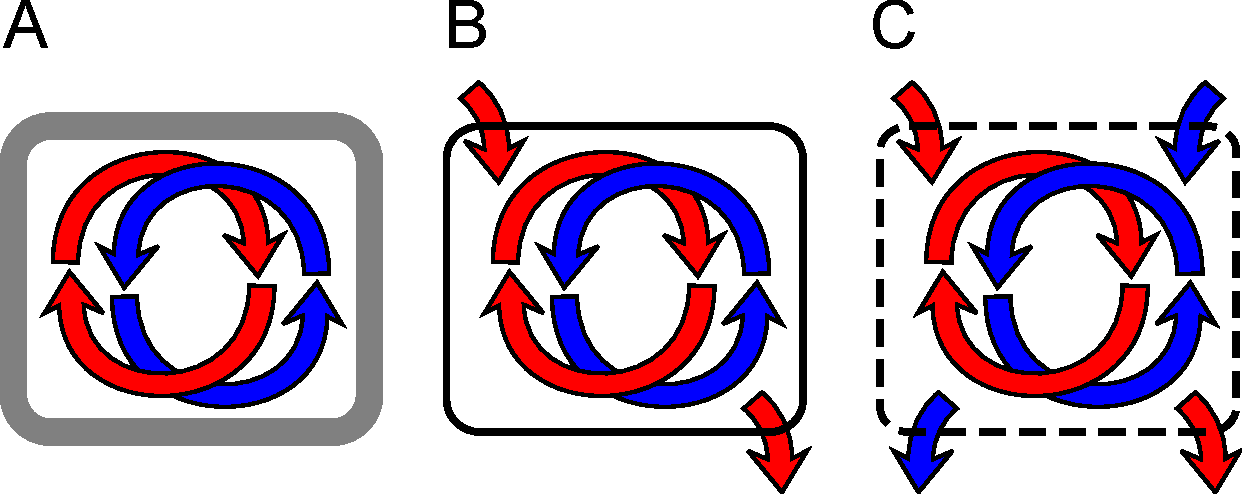
\includegraphics[width=\linewidth]{Part_0/Chapter_Introduction/images/systems.pdf} 
% \end{center}
% \caption[Isolated, closed, and open systems]{Isolated (A), 
% closed (B) and open (C) systems. 
% Red arrows represent energy flows. 
% Blue arrows represent material flows.}
% \end{figure}

\begin{table}
\caption[Hierarchy of systems]{Hierarchy of systems.\cite{Boulding1956}}
\begin{tabular}{r@{\hspace{1em}}l@{\hspace{1em}}l@{\hspace{1em}}l}
\toprule
\textbf{Level}	& \textbf{Description}	&	\textbf{Characteristic}	&	\textbf{Examples}	\\
\midrule
1	&	Structures	&	Static, spatial frameworks &	Atom, crystal, bridge	\\
2 & Clockworks & Predetermined motion	& Solar system, clocks, machines\\
3 & Control & Closed-loop feedback control mechanism & Heater with thermostat \\
4 & Open systems & Structurally self-maintaining	& Cells	\\
5	& Genetic systems & Community of cells & Plants	\\
6	& Animals	&	Nervous system, self-awareness & Birds and beasts	\\
7 & Humans & Self-consciousness, knowledge,
language & Human beings	\\
8 & Socio-cultural systems	&	Roles, values, communication &	Family, community, society	\\
9	&	Transcendental systems	&	Beyond our knowledge	&	Religion	\\
\bottomrule
\end{tabular}
\label{tab:hierarchy}
\end{table}

%%%%%%%%%%	Mechanistic	%%%%%%%%%%
\subsection{Traditional mechanistic view of economy}
\label{sec:mechanistic}
%%%%%%%%%%

The classical school of economics flourished during the Enlightenment
when Newton's clockwork universe was ticking along nicely,
physicists were beginning to build an understanding of
energy and its conservation, and
physicians and biologists were beginning to understand
the workings of the human body,
in particular the circulatory system.\footnote{William
Harvey is normally credited with the first anatomically
accurate description of the circulatory system, 
published in 1628.\cite{Harvey1889}
}
Most cultures were agrarian,
depending largely on land for food
and muscle power to get things done.
Agriculture was still at the whims of nature and
a sense of stewardship was still largely prevalent.
Economists were largely preoccupied with delineating
the main factors of production (land, labor and capital)
and their influence on economic output.

The neo-classical school of economics 
was born out of the fire of the Industrial Revolution.
Thermodynamicists were outlining theories on 
heat cycles and equilibrium processes allowing
the development of more efficient engines.
Machines were changing everything.
For the first time in history,
nature could be bent to the will of humans.
New vistas of experience (and riches) were
opening up in the New World.
The bounties of nature were there for the taking.

Figure~\ref{fig:perp_motion_1} 
depicts the traditional model of the economy,
represented in mainstream \emph{Principles of Economics} texts.
%Traditional economic flow accounting examines gross payments 
%from the household sector to the production sector 
%for goods and services, 
%the flow of payments from the production sector 
%to the household sector for wages and rents, 
%and the reciprocal flows of goods \& services 
%and factors of production. 
Goods and services flow from the production sector
to the household sector (consumption)
in exchange for payments.
The factors of production (labor, capital)
flow from the household sector to the
production sector in exchange for wages and rents.
Attention is primarily focused on the circular flow
of money (dashed line) which is
is often described in reference to 
the ``circular'' flow of blood around the body.
Hence we often speak of money as the
``lifeblood'' of the economy.

This traditional model of the economy is unashamedly mechanistic.
General equilibrium models of the economy~\cite{Walras1892, Walras1993}
borrowed directly from classical physics' models of 
mechanical equilibrium.\cite{Ingrao1990}
Markets specifically,
and the economy more generally,
are seen as being in ``balance.''

Additionally,
the traditional view of the economy~(as
depicted in Figure~\ref{fig:perp_motion_1}),
in much the same fashion as our naive picture of
the circulatory system,
is represented as separate from its environment.
``Blood'' circulates around the economy
with no need to interact with the rest of the universe.
Although the biosphere is shown in
Figure~\ref{fig:perp_motion_1}, 
it is rarely represented in mainstream economic texts. 
In mainstream economics, 
the economy is implicitly and figuratively separate from 
the material world within which it operates.
The traditional economic model is presented as 
an \emph{isolated} system, 
independent from flows of materials and energy 
to and from the biosphere.
All of the necessary factors to keep the economy
running exist within its confines.
Because these physical elements of the biosphere are absent from economic models,
the physical constraint they place on the allocation of resources, distribution of outputs, and 
scale of an economy are outside the scope of traditional economic discussion.
Because the economy is independent of any other processes
(floating in the void),
there is no effect of changing the scale of the economy.
Hence, economic growth has no associated costs.
If growing the economy can be shown to have any
societal benefits whatever,
we pursue the moral imperative for economic growth.
This moral imperative for economic growth 
combined with the expansionist vision of the pioneers
leads to the ``cowboy economy''
where everything is up for grabs.\cite{Boulding1966}

The next section will explore some problems with this
optimistic view.
%Although the Biosphere is represented in
%Figure~\ref{fig:perp_motion_1} 
%here, it is rarely represented in mainstream texts. 



\begin{figure}[!ht]
\centering\
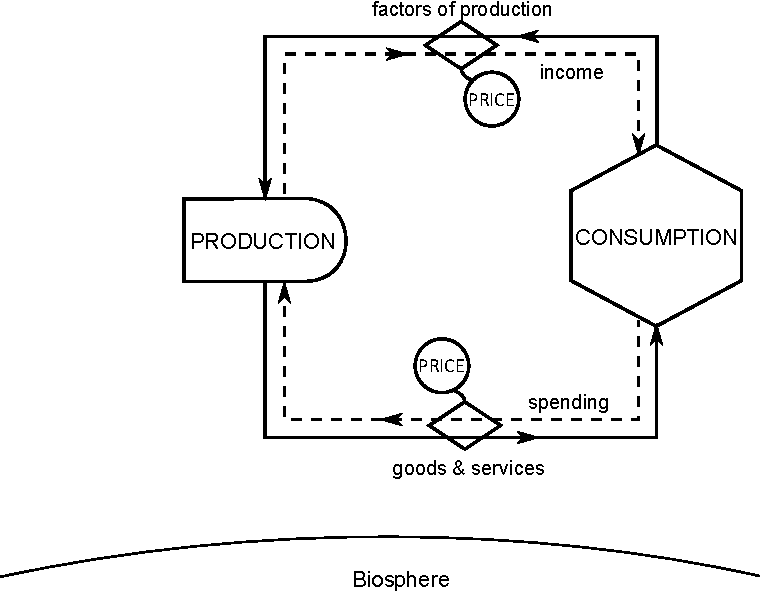
\includegraphics[width=\linewidth]{Part_0/Chapter_Introduction/images/Perpetual_motion_1.pdf}
\caption[The traditional economic model of the economy]{The economy 
is represented as a circular flow of goods and services between two sectors. 
The producers manufacture goods and services 
by taking in labor and capital. 
Consumers exchange labor for wages 
which are used to purchase 
the goods and services of the producers.}
\label{fig:perp_motion_1}
\end{figure}

%%%%%%%%%% Resource metaphors %%%%%%%%%%
\subsection{Economic models that include resource inputs}
\label{sec:metaphor_resource}
%%%%%%%%%% 

Thermodynamics tells us that all physical processes require
a transfer of energy.
Because Figure~\ref{fig:perp_motion_1} has no flow of energy
to the economy,
we may consider it a perpetual motion machine
of the \emph{first kind}:
it produces work without the input of energy and
thus violates the first law of thermodynamics---the 
law of conservation of energy.\cite{Rao2004}
The real circulatory system is connected to the lungs,
from where it takes in oxygen,
and to the digestive system, 
where it takes in processed food,
which are passed to the cells throughout the body.
This is a major function of the blood:
to act as an intermediary between the input of energy
and material resources,
the food we eat and air we breathe,
and the internal working of the body.
The circulatory system is necessarily connected 
to its environment and circulates energy and materials
that have been extracted from it.
%**** The rest of this paragraph needs to be thought about.
%A rewrite for clarity may be necessary.---MKH ****
%An intermediary is necessary because 
%the energy and material resources
%% and assimiliative capacity of the biosphere 
%required to run the economy are outside the model.
The economy as an isolated system
represents a ``perpetual motion machine,'' % chktex 38
seemingly able to operate indefinitely with 
no binding constraints.
Connecting the economy to the environment
by the necessity for (particularly) energy
resources raises issues for the indefinite
continuity of economic growth.

%**** This paragraph seems awkward to me.
%Possibly rewrite.---MKH ****
Proponents of the traditional, 
economy-is-all viewpoint fought back
by appeals to \emph{substitutability}.
A particular material (oil) may be in short supply,
but our technological expertise---which expands
as the economy grows---will allow us to substitute
another resource (coal) for it.
Substitution may continue indefinitely so,
goes the story,
in the final analysis the only limiting resource is
human ingenuity.\cite{Simon1981, Simon1998}

This assumption was thrown into stark relief following the oil
shocks of the Seventies.
Suddenly the global economy was thrown
into reverse for lack of one fundamental resource.
The necessity of including,
at the very least,
energy resources into the economic picture
spurred the efforts of early (net) energy 
analysts.\cite{Gilliland1975, Chapman1976}
%**** Unclear whether Figure~\ref{fig:perp_motion_2}
%deals with a closed or open system. 
%Is it allows energy or materials to flow through?---MKH ****
Figure~\ref{fig:perp_motion_2} depicts the traditional
economic model updated to account for 
resource flows from the biosphere
into the economy.
The economy has changed from an \emph{isolated}
system into an \emph{closed} system,
since only energy inputs have been accounted.

The metaphor for such a model is still very much
a mechanistic one.
This mechanistic description lends itself to a view of
the economy,
much like the engines of the Industrial Revolution,
as well-behaved and amenable to control.
Machine metaphors abound in our economic discussions.
We speak of the ``fueling'' the ``economic engine'' 
lest it should ``stall.''~\cite{Liu2012}
Like an engine, the economy is  assumed 
to be resilient to small and even quite large perturbations.  
It can either self-correct, 
or be corrected with adjustments to
a few predictable policy levers. 
Additionally, the biosphere is relegated to the position
of a provider of resources;
the larder of the economy.\cite{Norgaard2010}

\begin{figure}[!ht]
\centering\
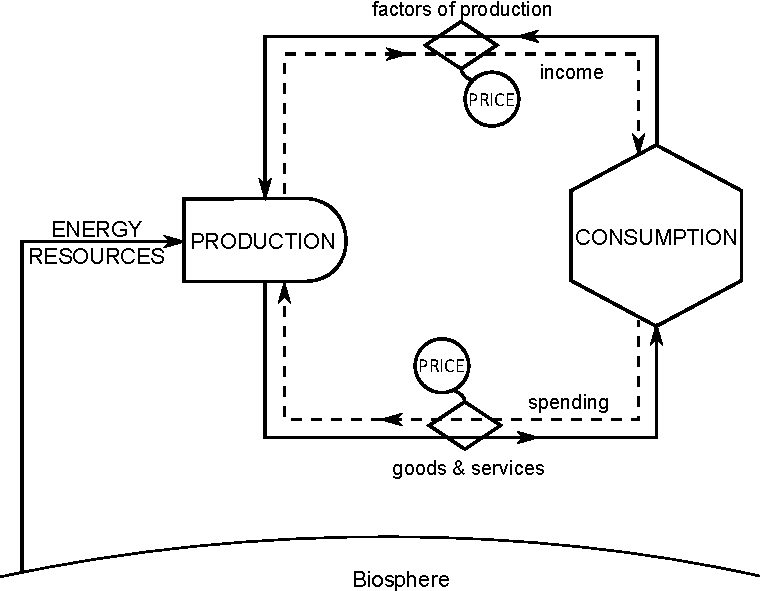
\includegraphics[width=\linewidth]{Part_0/Chapter_Introduction/images/Perpetual_motion_2.pdf}
\caption[The traditional model supplemented with resource inputs]{Energy 
and material input output analysis has included the flows into the economy from the environment.
This may be considered a perpetual motion machine 
of the second kind.
%*** MCD---SHOULD FLOW FROM `RAW RESOURCES' ALSO GO STRAIGHT INTO CONSUMPTION?***
%**** Should ``Raw Resources'' be replaced by ``Energy?'' 
%Should waste heat be added?
%If this is a closed system, you can have energy flows, but not material flows.---MKH ****
}
\label{fig:perp_motion_2}
\end{figure}

%%%%%%%%%% Metabolic	%%%%%%%%%% 
\subsection{The metabolic economy}
\label{sec:metabolic}
%%%%%%%%%% 

The cowboy economy soon depletes resources.
The consumption of resources also leads to wastes.
The question arises as to ``what to do with these wastes?''
The traditional economic view sees these wastes as
an anomaly to the normal functioning of the economy.~\cite{Ayres1969}
Thermodynamics takes a different stance.

According to the Second Law of Thermodynamics\index{Second Law of Thermodynamics},
all real-world processes involve the degradation
of material and especially energy resources
and the creation of entropy.
High quality (low entropy) material and energy come in,
low quality (high entropy) material and energy go out.
The depiction in Figure~\ref{fig:perp_motion_2} 
can be classified as a perpetual motion machine
of the \emph{second kind}:
it perfectly converts energy resources into 
work~(useful services) without generating
any entropy,
in violation of the second law of thermodynamics.
Since the generation of high entropy~(low quality)
output is a \emph{necessary} feature of \emph{all} processes 
(including economic processes)
then the generation of wastes is a normal feature of
economic processes,
not an anomaly.
Within a closed system, such as the earth,
these wastes soon accumulate,
necessitating the change to a ``spaceship'' economy,
wherein account is made of the waste outflows of
the economy.

In Figure~\ref{fig:metabolic_economy},
the production and consumption sectors both produce
waste flows which must be assimilated by the biosphere.
Our circulatory system also circulates carbon dioxide
(waste from the consumption of food-fuel with oxygen)
and urea (waste from protein catabolism) for extraction
and exchange to the environment.

Environmental Economics, as a sub-discipline, 
expands traditional economic models by recognizing the
valuable role played by the environment in supporting the 
economy and attempting to place value in those services.
However, even with this expanded model, 
the simplifying metaphor,
that of an engine,
remains intact. 
% Simply measuring these input and output flows is not enough.
Predominantly linear relationships of inputs and outputs rule the day. 
Successful management of  local pollution, such as SO$_2$, 
through environmental legislation
is a positive result of this expanded model.
However, systemic events resulting from reinforcing feedback loops 
or from events occurring outside historical experience 
cannot be modeled and are not predictable. 
The 2007 global financial crisis is an example of one such systemic event.~\cite{Economist2010}
The 1930's dust bowl is an example of a systemic event. 
It was one of the greatest man-made environmental disasters, 
arising from unexpected, non-linear 
results of widely accepted traditional farming practices, 
implemented in a new, and unknown ecosystem.~\cite{Lockertz1978} 

%We must convert our understanding from that of a machine,
%albeit one where we account both inputs and outputs,
%to that of an organism.

Ecological economists, 
in the tradition of Herman Daly, 
have begun to update the traditional models.\cite{F-K2003} 
In ecological economics texts, 
the economy is 
represented as a \emph{open} system. 
The guiding metaphor for this kind of 
economic model is an \emph{organism}.
The blood serves a self-regulatory, homeostatic role
by transporting hormones. 
Like an organism,
the economy metabolizes energy and materials 
that it receives from natural resources into forms 
usable for human purposes.
The economy's behavior is non-linear and chaotic,
but also self-regulating.
Models and accounting systems are being
developed to describe ``society's metabolism.''~\cite{F-K1998, 
ConAccount1998, Giampietro2000, Daniels2001, Ayres2002, 
Haberl2001, Giampietro2013}

Empirical measurements are necessary to support
(or dispute) scientific theory and models.
Accounting frameworks and methodologies are necessary
to facilitate measurement.
The following sections outline attempts to
account flows of economic factors through the
economy. 
The first (Section~\ref{sec:IO_basic}),
looks at traditional input-output models, 
which assume that the economy is an isolated system 
and track only flows of money.
The second (Section~\ref{sec:IO_resource},
looks at the development of the energy input-output methodology
(an extension of the traditional method),
which assumes that the economy is open to inputs of energy.
The third (Section~\ref{sec:IO_waste}),
looks at further extension of the input-output methodology
to include other material extractions from the biosphere and also
to track discharges from the economy back into the biosphere.
In the fourth (Section~\ref{sec:IO_dynamic}),
we give a justification for a further extension of the input-output
methodology to include,
not only flows (of physical materials and money),
but also \emph{accumulations} of these items
in economic sectors.
%**** Within which type of model: open, closed, or isolated?---MKH ****
%
%
%**** Metaphor Sources and Cites BRH recommends:
%
%
%1. Norgaard, Richard B. “Ecosystem Services: From Eye-Opening Metaphor to Complexity Blinder.” Ecological Economics 69, no. 6 (April 2010): 1219--1227. \url{doi:10.1016/j.ecolecon.2009.11.009}. **** BRH says---this article is useful for helping dispel the notion that the econ models need to simply 
%add in flows of ecosystems on the front and back end of the traditional model---and keep it a simple linear model. The usefulness
%of using an ecological model is that in addition, it captures the systemic complexity of the economy as well. ****
%
%
%2. McCloskey, Deirdre N. If You’re so Smart: The Narrative of Economic Expertise. Chicago: University of Chicago Press, 1990. *** BRH 
%If we are talking at all about metaphor in economics, we have to look at Dierdre McCloskey. (You can read the first chapter here---see source for link).
%%%% http://books.google.com/books?printsec=frontcover&vid=ISBN0-226-55670-0#v=onepage&q&f=false). 
%She is 
%the iconoclast in economics and this book is one place she talks about how economists misuse
%metaphor and story to make their point more than rigor. (note: she changed her
%name and her gender in the early 90's, this book was originally published as Donald McCloskey).



\begin{figure}[!ht]
\centering\
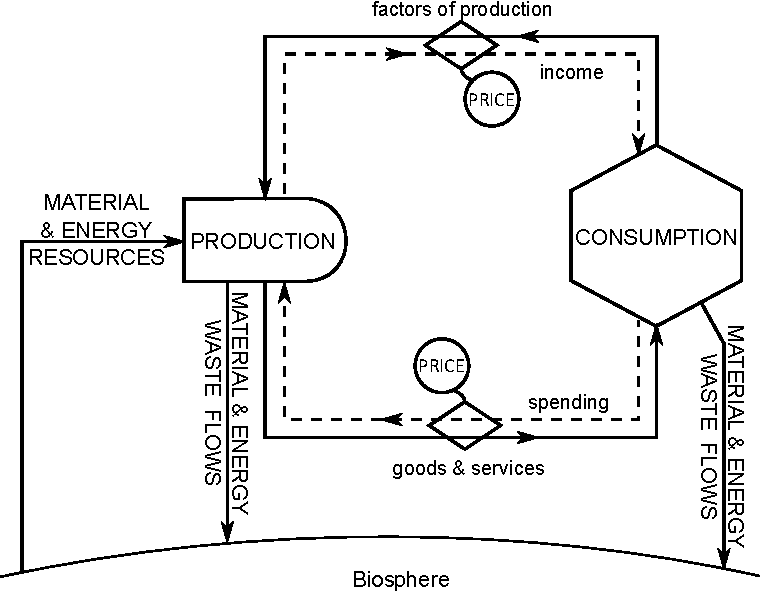
\includegraphics[width=\linewidth]{Part_0/Chapter_Introduction/images/PERKS.pdf}
\caption[A comprehensive biophysical (?) model of the economy]{A comprehensive model 
of the economy, fully consistent with the laws of thermodynamics 
must include degraded resources (waste) expelled 
to the environment as a necessary consequence of economic activity.}
\label{fig:metabolic_economy}
\end{figure}

%**** I think we need some type of transition to accounting here.---MKH ****

%%%%%%%%%% I-O History	%%%%%%%%%% 
\section{Brief history of input-output (I-O) modeling}
\label{sec:history}
%%%%%%%%%% 

Input-output analysis, developed by Wassilly Leontief in the 1930s 
as an extension to the work of Quesnay and Walras~\cite{Leontief1936}, 
is of primary importance in national accounting. 
The method allows determination of the flows of value through
an economy as well as, 
among other things, 
calculation of a nation's gross domestic product (GDP), 
today's prevailing measure of economic activity.



%%%%%%%%%% Basic I-O		%%%%%%%%%% 
\subsection{Basic I-O method}
\label{sec:IO_basic}
%%%%%%%%%% 

The basic premise of the I-O method, 
as depicted in Figure~\ref{fig:basic_unit}A, 
is that each economic sector takes in factors of production 
from other sectors (and possibly itself) 
to produce an economic good at some rate. 
For example, the automotive sector takes in steel, rubber, glass, etc. 
and produces a number of cars per year. 
In contrast to high-level economic growth models 
that include only a few factors of production (such as land, capital, and labor), 
the I-O analysis technique allows many differentiated factors of production 
and raw material feedstocks.\cite{Costanza:1980ww} 
In I-O frameworks, each factor of production 
is considered to be a output from a sector of the economy. 
As will be discussed later,
%****MAKE SURE TO DISCUSS THIS LATER!****, 
the traditional primary factors of production (land, capital, and labor) 
are not \emph{flows} into the production processes. 
Rather, they are \emph{stocks} that, when present, 
allow factors of production (steel, rubber, and glass) 
to be transformed into final products (automobiles). 
The quantity and quality of these stocks 
determine the quantity and quality of their flow of productive services.

\begin{figure}[!ht]
\centering\
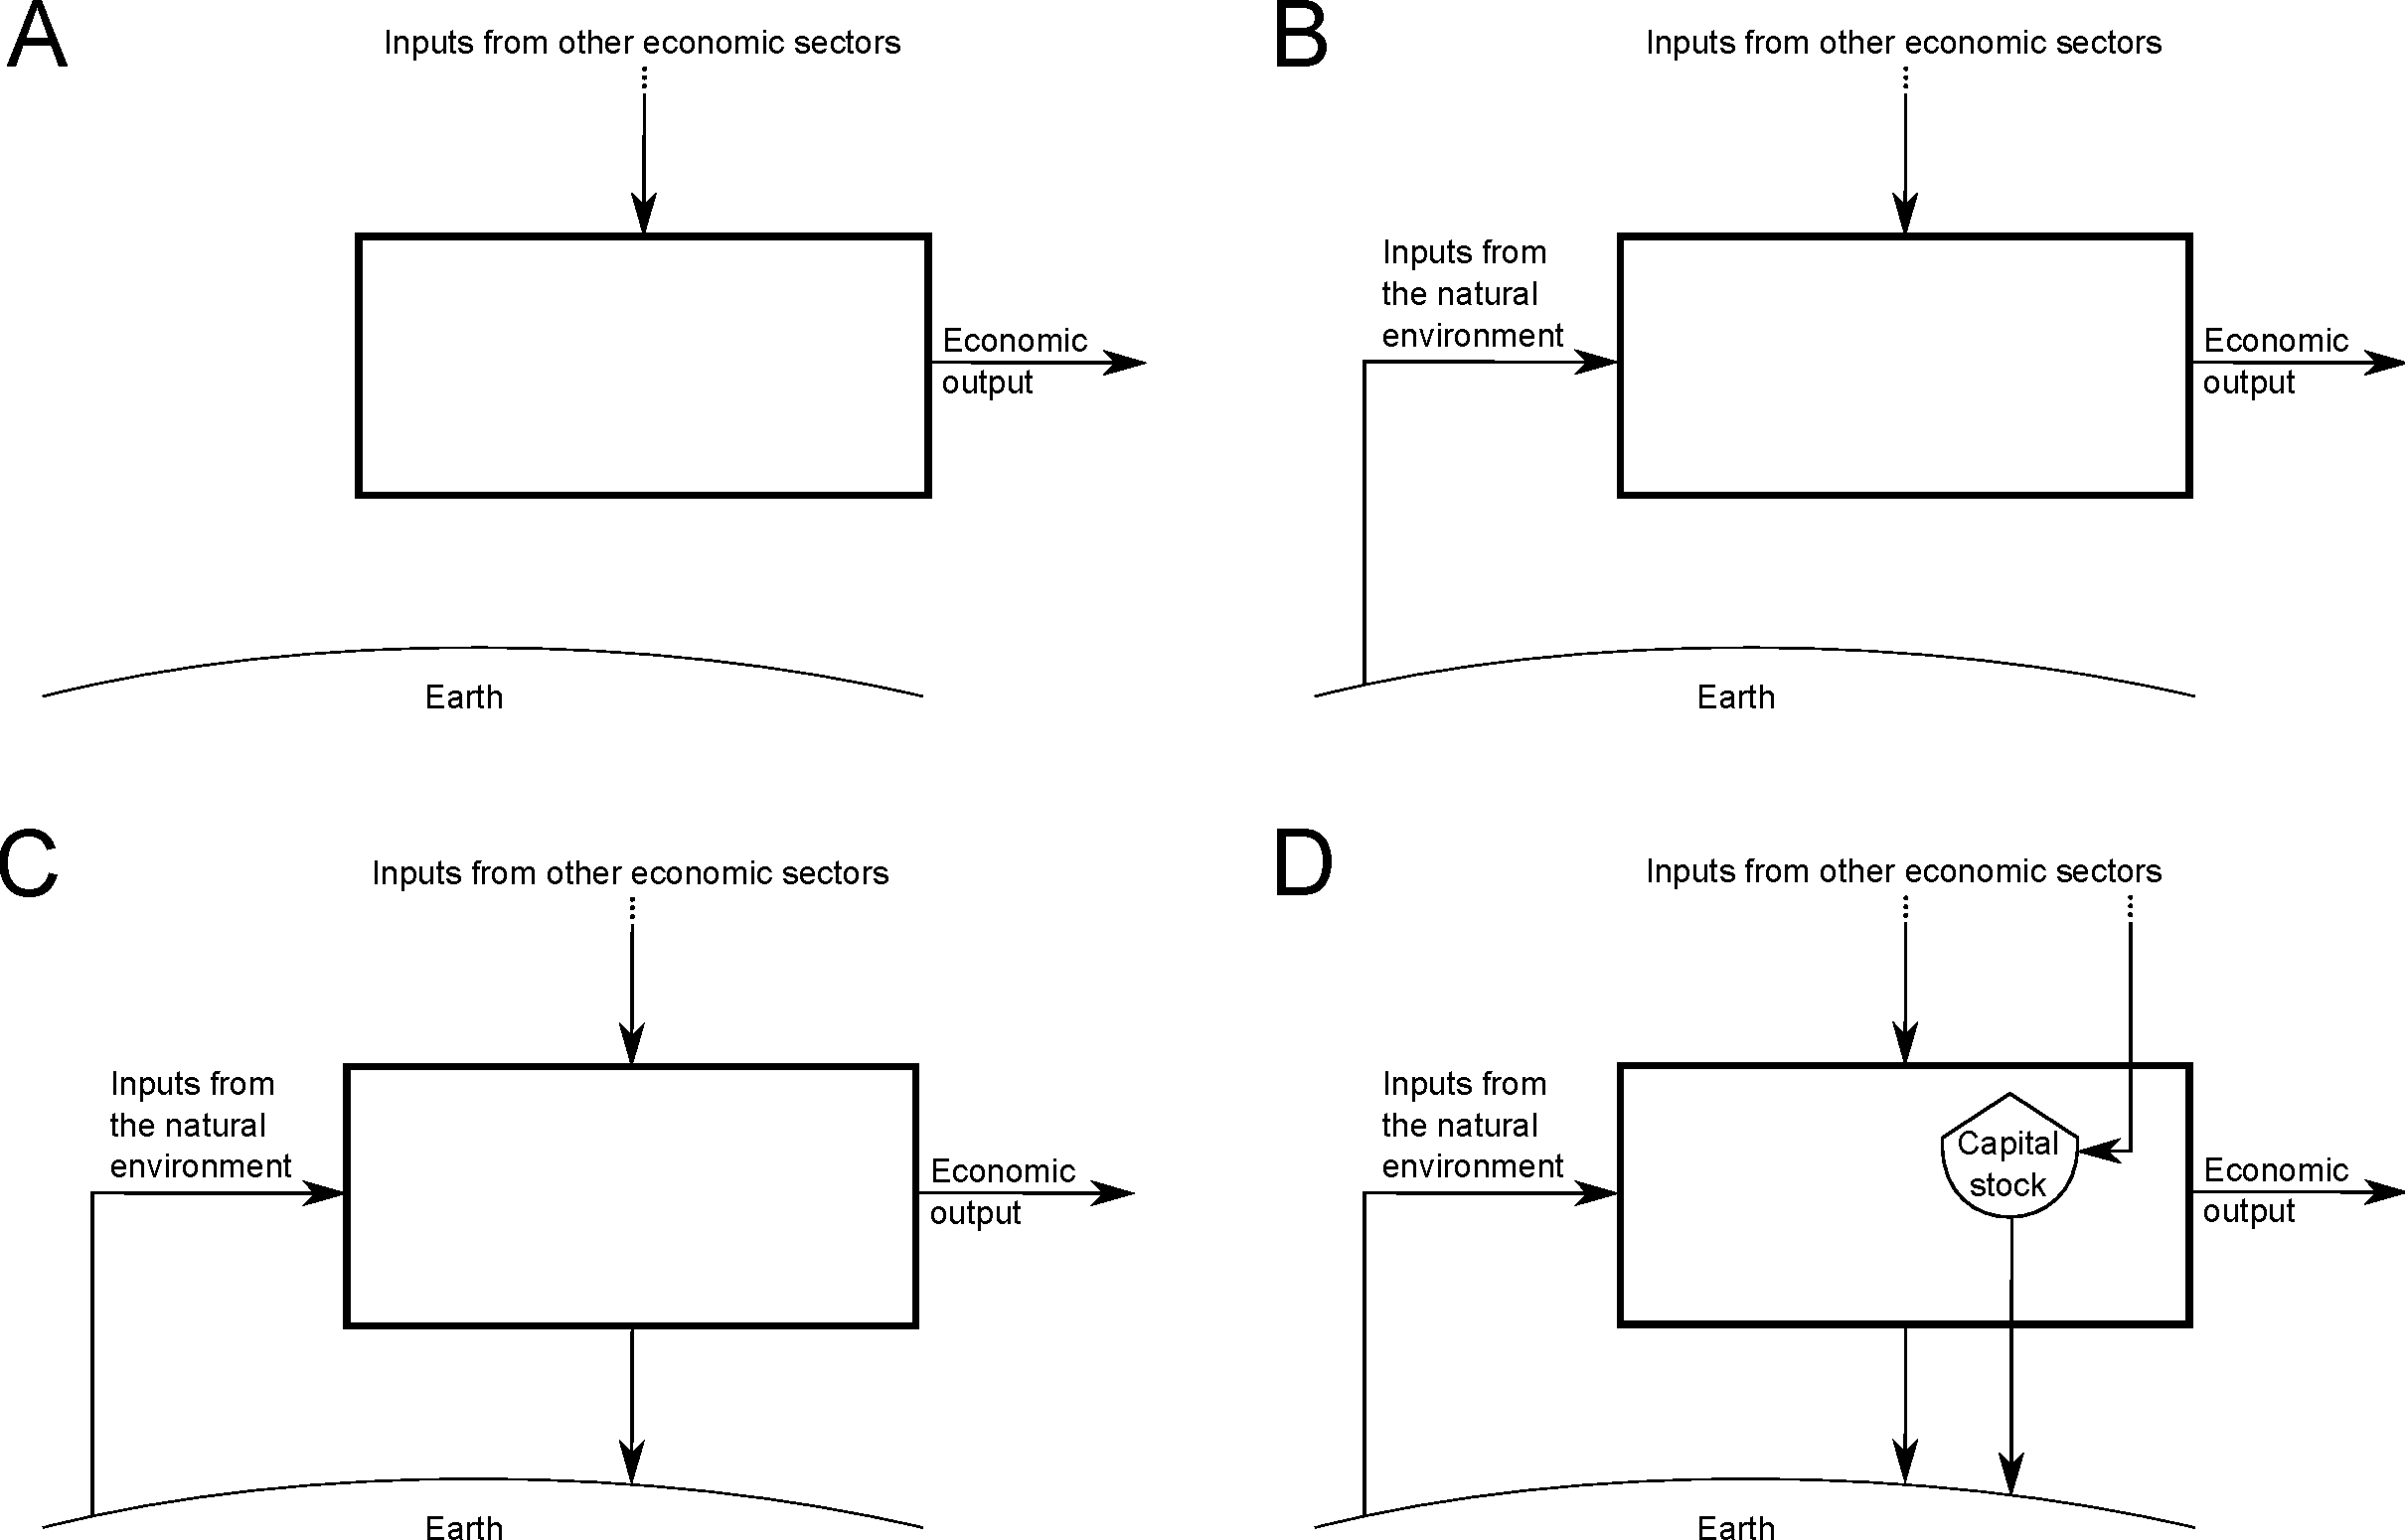
\includegraphics[width=\linewidth]{Part_0/Chapter_Introduction/images/Basic_unit_square.pdf}
\caption[The basic unit of input-output modeling]{The basic unit 
of input-output modeling: 
\textbf{A} the standard economic approach includes only transactions 
among sectors of the economy; 
\textbf{B} the energy input-output approach models inputs 
from the natural environment outside the economy as factors of production; 
\textbf{C} including waste flows to the environment makes the model physically consistent and;
\textbf{D} the method presented here accounts also for accumulation
in capital stock, $K$, of embodied energy within materials in economic sectors. 
%****SHOULD WE HAVE THE LABEL ``K'' IN THE ACCUMULATION, OR JUST HAVE THE TANK?***
%**** MY SENSE IS THIS HAS BEEN TAKEN CARE OF---MCD 01/30/2014 ****
}
\label{fig:basic_unit}
\end{figure}

%%%%%%%%%% Resource I-O	%%%%%%%%%% 
\subsection{I-O method including inputs from the biosphere}
\label{sec:IO_resource}
%%%%%%%%%% 

The oil shocks of the Seventies spurred great interest in
the important role of energy in economic production.
In addition to the productive services 
provided by flows of capital and labor,
a flow of energy\footnote{Or, more precisely, 
the degradation of an exergetic gradient/destruction of exergy.} 
is required for economic activity. 
These energy flows originate from the natural environment, 
recognition of which provoked researchers from fields of 
net energy analysis\index{net energy analysis} (NEA), 
to extend the traditional~(Leontief\index{Leontief}) 
input-output framework 
to include important 
energy flows from the environment, 
developing an energy input-output\index{energy input-output} 
(EI-O) model
as depicted in Figure~\ref{fig:basic_unit}B.\cite{Carter1974,
Bullard1975,Bullard1976a,Herendeen1978,Costanza:1980ww,
Casler1984,Joshi:1999uw,Suh2009}
While the Leontief I-O approach relies exclusively 
on monetary units to represent value flows 
among sectors of an economy, 
the key insight of the EI-O framework 
is to rely upon physical units 
(especially energy units of joules) 
to represent some of the flows among economic sectors. 
In doing so, 
energy intensities of monetary flows can be estimated. 

However,
as we discussed above,
resource inputs are only one side of the coin.
According to thermodynamics,
all acts of production (requiring inputs from the biosphere)
are simultaneously acts of consumption,
degrading high quality inputs into wastes to be 
discharged back into the biosphere.


%\section{Issues of resource quality}
%
%[DO WE NEED THIS SECTION? IT FEELS LIKE WE SHOULD MOVE FROM THE PREVIOUS SECTION WHEREIN WE CLEARLY DEMONSTRATE THE NEED FOR OUR WORK TO BEGINNING THE PROCESS OF DEVELOPING THE METHOD. IF WE WANT TO KEEP THIS SECTION, WE SHOULD DO A BETTER JOB AT SHOWING WHY IT IS NEEDED. WE SHOULD POINT BACK TO BULLARD AND HERENDEEN AND SAY THAT THEIR METHOD DOESN'T ACCOUNT FOR DECREASING RESOURCE QUALITY AND WHY A METHOD IS NEEDED THAT DOES ACCOUNT FOR DECLINING RESOURCE QUALITY. --MKH] 
% [MCD---I'm going to steal this paragraph for the Unfinished Business chapter.]
%Raw material and energy resources must first be extracted from the natural environment before they may be utilized in the economy to provide goods and service to society. Despite increasing levels of technological efficiency, for example in consumer goods such as refrigerators and cars, evidence shows that the energy intensity of primary resource extraction, i.e. the energy required to extract raw materials from the environment, has been steadily increasing over the last fifty years \cite{Hall1986, Mudd2010, Brandt2011}. This increasing energy requirement for primary extraction means that less \textit{net energy} is available for downstream uses. If this decline in net energy availability outpaces technological advances in energy efficiency, there may be deleterious impacts on the economic output of the economy.

%%%%%%%%%% Waste IO	%%%%%%%%%% 
\subsection{I-O methods including resource inputs and waste flows}
\label{sec:IO_waste}
%%%%%%%%%% 
%**** MCD---needs work ****
Now that the global economy is experiencing the pressure of physical constraints, 
the necessity for a more comprehensive model, 
and collection of data to estimate it,
is emerging. 
A number of disciplines including
material flow analysis (MFA), 
industrial ecology (IE), and 
life-cycle assessment (LCA) 
have developed further extensions of the EI-O
framework to account for energy and material flows
both into and out of the economy from the biosphere.
Motivated by concerns over environmental impacts
(especially climate change),
the primary focus of such efforts has been on
tracking flows of materials
(especially greenhouse gases)
into the biosphere
rather than on resource depletion.\cite{ConAccount1998,
Lenzen1998, Hoekstra2003, Bailey2004, Pedersen2006, Turner2007}
%**** Mik---Reference needs to be fixed. ****
This extended approach is depicted in Figure~\ref{fig:basic_unit}C. 

% ***** MCD----add this somewhere ****
The making industries related to extraction, 
refining, and utilities mark the entry point for 
materials extracted from the biosphere into the economy. 
These three industries (extraction, refining, and utilities) 
are the first three industries listed in the 
NAICS (North American Industry Classification System) 
that the BEA uses to track economic information.~\cite[p.~25]{Lawson2002}
%****BRH add cite (Law- son and et al. 2002, 25). ****
**** MCD---Becky, is this the right ref? ***
Conversely, consumption, with associated waste
discharge, occur from all sectors of the economy.
But why do we have consumption?
Boulding tells us that consumption is the 
real cost of living in a physical world;
that there is,
\begin{quotation}
no particular virtue in consumption. 
It is, unfortunately, 
a necessary incident in the business of living. 
We cannot eat without destroying food; 
we cannot walk without destroying shoes; 
we cannot drive without destroying gasoline, 
tires, and cars; and so on.\cite[p.2]{Boulding1945}
\end{quotation}
In a sense then,
it is the existence of physical objects within our economies
(and their subsequent degradation)
that is the driver of consumption.
As such,
to truly understand our economies and the 
flows of materials through them,
we must account the physical stocks within them.


%%%%%%%%%% Dynamic IO		%%%%%%%%%% 
\subsection{An I-O method for dynamic (transient) economic analysis}
\label{sec:IO_dynamic}
%%%%%%%%%% 

Both the original Leontief I-O framework 
and the extensions cited above 
assume steady-state conditions in an economy, 
i.e., flows of value and material into 
and out of each economic sector are in balance. 
Dynamic or transient behavior 
of the economic system is not considered. 
Thus, there is no accumulation of economic factors 
or embodied energy within any of the sectors. 
The analysis techniques provide ``snapshots'' 
of economic activity at an instant in time.

%[MIK'S NEW ADDITION]
Assuming no accumulation of materials, 
within economic sectors or society itself, 
is tantamount to assuming that \emph{all} material flows 
through the economy are directed toward 
the production of non-durable goods. 
However, evidence of the durability of goods 
and the accumulation of materials surrounds us. 
Furthermore, 
energy was required to both fabricate and emplace 
the durable goods and infrastructure of modern economies. 
(The energy it took to create the durable goods and infrastructure 
can be considered ``embodied'' within the built environment, 
a point to which we will return in detail later). 
As Georgescu-Roegen notes, 
``in the everyday world one cannot possibly cross a river 
only on the flow of maintenance materials 
of a non-existent bridge.''~\cite{G-R1975}

Analysis methods that neglect the accumulation 
of materials and embodied energy 
in the durable goods and infrastructure 
of the everyday world lack explanatory power. 
Such models can tell us at what rates materials 
and energy are required 
to \emph{use} our built environment. 
But, such models cannot tell us \emph{how} 
the built environment came to be 
(and how much energy was required to construct it) 
or \emph{why} flows of goods are needed to maintain it. 
To use Georgescu-Roegen's imagery, 
models that neglect accumulation fail to explain 
why we need any material flows to maintain a non-existent bridge. 
Stocks of accumulated materials 
(capital, appliances, even people) 
are drivers of demand. 
It is to service their needs and wants that we put the economy to work. 

Georgescu-Roegen distinguishes two types of economic
inputs: \emph{flows} which are the resources (such as cloth and thread)
to be transformed into final products (shirts) 
% **** What about $\dot{S}$ flows, too?----MKH **** 
and \emph{funds}---stocks
(such as needles) that must be present in order to facilitate the transformation.
Confusing the two categories could lead to some painful 
consequences!~\cite{G-R1970}
Daly makes a similar distinction between \emph{material} 
and \emph{efficient causes}.\cite{Daly2006}
A full model of the economy must account the 
stocks~(funds, efficient causes) that give rise
to the flows~(material causes).

Because economic activity requires energy, 
we need to understand the way energy flows through economies. 
The steady-state I-O techniques of Bullard, Herendeen, 
and others~\cite{Bullard1975,Herendeen1978} 
offer a means to that end. 
We contend, however, that these techniques 
need to be extended and modified 
to include transient effects 
that arise when durability of goods and infrastructure 
(and associated embodied energy) are considered. 
When accumulation is not accounted for,
the assumption is that all flows in and out balance
instantaneously.
Imagine a bath tub where the water flowing in
through the tap is exactly balanced by the water
flowing out the plughole.
The state of the system 
(the amount of water within the bath) is 
fixed---therefore we say the system is in
steady-state.
Imagine instead a growing baby.
The inputs of food and other materials,
though small compared to an adult,
exceed the output of excreta
(gas, solid and liquid).
While this may be hard for new parents to believe
(how can there be possibly be more going in than is coming out!),
it is simply this imbalance that induces the growth of the baby.
Materials accumulate within the baby's body.
Obviously, 
this imbalance (and the subsequent growth induced)
slows as the child grows up to adulthood.
Nevertheless,
adults still maintain the ability to accumulate
materials.
We can gain (or lose) weight;
a fact to which any yo-yo dieter will readily attest.

Steady-state systems are unable to change
their internal state.
Real systems are rarely in steady state.
As such, our economic models
and associated accounting frameworks
need to be able to deal with dynamic systems
that are not in steady-state---they must
be able to account accumulation within the economy.

In this manuscript, we develop a physical input-output, 
matrix-based framework for modeling multi-sector economies, 
in the tradition of Georgescu-Roegen's ``flow-fund'' 
model.\cite{G-R1979a, G-R1979b} 
%**** Need to re-cast in metabolism language!!!! **** 
The method presented takes a decidedly thermodynamic approach
to extend the techniques of Bullard, Herendeen, and others 
to account for accumulation of goods and embodied energy. 
This framework allows us to see how energy 
and materials flow through the economy, 
as well as where embodied energy accumulates in the economy.
Real economies, 
much like babies,
grow and develop.
Their internal structures are dynamic,
undergoing change and transitions.
We need to be able to understand these development
by understanding the underlying structural change.
The framework developed in this book
addresses that need.
%[NEED TO MAKE SURE WE ACHIEVE THIS LAST POINT]

%%%%%%%%%% Structure	%%%%%%%%%% 
\section{Structure of the book}
\label{sec:structure}
%%%%%%%%%% 

The remainder of this book is organized as follows. 
Part~\ref{part:matter} models flows of physical matter
through the economy.
Chapter~\ref{chap:materials} presents a discussion of material flows.
Flows of direct energy are discussed in Chapter~\ref{chap:direct_energy}, 
and a rigorous, thermodynamics-based definition of and accounting for 
embodied energy is presented in Chapter~\ref{chap:embodied_energy}.
In Part~\ref{part:values} we turn to non-physical flows through the economy. 
Flows of economic value are discussed in Chapter~\ref{chap:value}.
In Chapter~\ref{chap:intensity} we combine the results from 
Chapters~\ref{chap:embodied_energy}~and~Chapter~\ref{chap:value} to
calculate the energy intensity of economic production.
Part~\ref{part:implications} gives context to the framework developed in
Parts~\ref{part:matter}~and~\ref{part:values}.
Chapter~\ref{chap:implications} draws out some of the direct implications
of the results.
Chapter~\ref{chap:unfinished_business} looks at 
unfinished business: practical, conceptual, and theoretical issues
that arise in the development of this framework.
We finish off the book with a summary in Chapter~\ref{chap:summary}.

Throughout the methodological Chapters~(\ref{chap:materials}--\ref{chap:value}),
the framework is developed
through a series of increasingly-disaggregated
models of the economy (Table~\ref{tab:examplesABC}). 
In addition, we use the the US auto industry 
as a running example for application and discussion.
We choose the auto industry,
because it remains a large portion of most industrialized economies, 
because is very resource intensive,
because it has been used in the literature~\cite{Bullard:1978vd}
to illustrate input-output accounting methods, 
because its links with energy are obvious,
because its health is sensitive to disruptions in energy supplies, and
because it shows evidence of post-industrial decline (shrinking profit margins, etc.).


\begin{table}
\caption{Examples
used throughout this book}
\begin{center}
  \begin{tabular}{r @{\hspace{2em}} c @{\hspace{2em}} c @{\hspace{2em}} c @{\hspace{2em}} c}
    \toprule
    Example & Sector 0 & Sector 1 & Sector 2 & Sector 3 \\ 
	\midrule
    A & Biosphere	&	Society            & NA         & NA                 \\
    B & Biosphere	&	Final Consumption  & Production & NA                 \\
    C & Biosphere	&	Final Consumption  & Energy     & Goods \& Services  \\
  \bottomrule
  \end{tabular}
\end{center}
\label{tab:examplesABC}
\end{table}


\bibliographystyle{unsrt}
\bibliography{../../EROI_review_v2}


% Always give a unique label
% and use \ref{<label>} for cross-references
% and \cite{<label>} for bibliographic references
% use \sectionmark{}
% to alter or adjust the section heading in the running head
%% Instead of simply listing headings of different levels we recommend to let every heading be followed by at least a short passage of text. Furtheron please use the \LaTeX\ automatism for all your cross-references and citations.

%% Please note that the first line of text that follows a heading is not indented, whereas the first lines of all sequent paragraphs are.

%% Use the standard \verb|equation| environment to typeset your equations, e.g.
%
%% \begin{equation}
%% a \times b = c\;,
%% \end{equation}
%
%% however, for multiline equations we recommend to use the \verb|eqnarray|
%% environment\footnote{In physics texts please activate the class option \texttt{vecphys} to depict your vectors in \textbf{\itshape boldface-italic} type - as is customary for a wide range of physical jects.}.
%% \begin{eqnarray}
%% a \times b = c \nonumber\\
%% \vec{a} \cdot \vec{b}=\vec{c}
%% \label{eq:01}
%% \end{eqnarray}

%% \section{section Heading}
%% \label{sec:2}
%% Instead of simply listing headings of different levels we recommend to let every heading be followed by at least a short passage of text. Furtheron please use the \LaTeX\ automatism for all your cross-references\index{cross-references} and citations\index{citations} as has already been described in Sect.~\ref{sec:2}.

%% \begin{quotation}
%% Please do not use quotation marks when quoting texts! Simply use the \verb|quotation| environment -- it will automatically render Springer's preferred layout.
%% \end{quotation}


%% \section{section Heading}
%% Instead of simply listing headings of different levels we recommend to let every heading be followed by at least a short passage of text. Furtheron please use the \LaTeX\ automatism for all your cross-references and citations as has already been described in Sect.~\ref{sec:2}, see also Fig.~\ref{fig:1}\footnote{If you copy text passages, figures, or tables from other works, you must obtain \textit{permission} from the copyright holder (usually the original publisher). Please enclose the signed permission with the manucript. The sources\index{permission to print} must be acknowledged either in the captions, as footnotes or in a separate section of the book.}

%% Please note that the first line of text that follows a heading is not indented, whereas the first lines of all sequent paragraphs are.

% For figures use
%
%% \begin{figure}[b]
%% \sidecaption
% Use the relevant command for your figure-insertion program
% to insert the figure file.
% For example, with the option graphics use
%% \includegraphics[scale=.65]{figure}
%
% If not, use
%\picplace{5cm}{2cm} % Give the correct figure height and width in cm
%
%% \caption{If the width of the figure is less than 7.8 cm use the \texttt{sidecapion} command to flush the caption on the left side of the page. If the figure is positioned at the top of the page, align the sidecaption with the top of the figure -- to achieve this you simply need to use the optional argument \texttt{[t]} with the \texttt{sidecaption} command}
%% \label{fig:1}       % Give a unique label
%% \end{figure}


%% \paragraph{Paragraph Heading} %
%% Instead of simply listing headings of different levels we recommend to let every heading be followed by at least a short passage of text. Furtheron please use the \LaTeX\ automatism for all your cross-references and citations as has already been described in Sect.~\ref{sec:2}.

%% Please note that the first line of text that follows a heading is not indented, whereas the first lines of all sequent paragraphs are.

%% For typesetting numbered lists we recommend to use the \verb|enumerate| environment -- it will automatically render Springer's preferred layout.

%% \begin{enumerate}
%% \item{Livelihood and survival mobility are oftentimes coutcomes of uneven socioeconomic development.}
%% \begin{enumerate}
%% \item{Livelihood and survival mobility are oftentimes coutcomes of uneven socioeconomic development.}
%% \item{Livelihood and survival mobility are oftentimes coutcomes of uneven socioeconomic development.}
%% \end{enumerate}
%% \item{Livelihood and survival mobility are oftentimes coutcomes of uneven socioeconomic development.}
%% \end{enumerate}


%% \paragraph{paragraph Heading} In order to avoid simply listing headings of different levels we recommend to let every heading be followed by at least a short passage of text. Use the \LaTeX\ automatism for all your cross-references and citations as has already been described in Sect.~\ref{sec:2}, see also Fig.~\ref{fig:2}.

%% Please note that the first line of text that follows a heading is not indented, whereas the first lines of all sequent paragraphs are.

%% For unnumbered list we recommend to use the \verb|itemize| environment -- it will automatically render Springer's preferred layout.

%% \begin{itemize}
%% \item{Livelihood and survival mobility are oftentimes coutcomes of uneven socioeconomic development, cf. Table~\ref{tab:1}.}
%% \begin{itemize}
%% \item{Livelihood and survival mobility are oftentimes coutcomes of uneven socioeconomic development.}
%% \item{Livelihood and survival mobility are oftentimes coutcomes of uneven socioeconomic development.}
%% \end{itemize}
%% \item{Livelihood and survival mobility are oftentimes coutcomes of uneven socioeconomic development.}
%% \end{itemize}

%% \begin{figure}[t]
%% \sidecaption[t]
% Use the relevant command for your figure-insertion program
% to insert the figure file.
% For example, with the option graphics use
%% \includegraphics[scale=.65]{figure}
%
% If not, use
%\picplace{5cm}{2cm} % Give the correct figure height and width in cm
%
%% \caption{Please write your figure caption here}
%% \label{fig:2}       % Give a unique label
%% \end{figure}

%% \runinhead{Run-in Heading Boldface Version} Use the \LaTeX\ automatism for all your cross-references and citations as has already been described in Sect.~\ref{sec:2}.

%% \runinhead{Run-in Heading Italic Version} Use the \LaTeX\ automatism for all your cross-refer\-ences and citations as has already been described in Sect.~\ref{sec:2}\index{paragraph}.
% Use the \index{} command to code your index words
%
% For tables use
%
%% \begin{table}
%% \caption{Please write your table caption here}
%% \label{tab:1}       % Give a unique label
%
% For LaTeX tables use
%
%% \begin{tabular}{p{2cm}p{2.4cm}p{2cm}p{4.9cm}}
%% \hline\noalign{\smallskip}
%% Classes & class & Length & Action Mechanism  \\
%% \noalign{\smallskip}\svhline\noalign{\smallskip}
%% Translation & mRNA$^a$  & 22 (19--25) & Translation repression, mRNA cleavage\\
%% Translation & mRNA cleavage & 21 & mRNA cleavage\\
%% Translation & mRNA  & 21--22 & mRNA cleavage\\
%%Translation & mRNA  & 24--26 & Histone and DNA Modification\\
%%\noalign{\smallskip}\hline\noalign{\smallskip}
%%\end{tabular}
%%$^a$ Table foot note (with superscript)
%%\end{table}
%
%% \section{Section Heading}
%%\label{sec:3}
% Always give a unique label
% and use \ref{<label>} for cross-references
% and \cite{<label>} for bibliographic references
% use \sectionmark{}
% to alter or adjust the section heading in the running head
%% Instead of simply listing headings of different levels we recommend to let every heading be followed by at least a short passage of text. Furtheron please use the \LaTeX\ automatism for all your cross-references and citations as has already been described in Sect.~\ref{sec:2}.

%% Please note that the first line of text that follows a heading is not indented, whereas the first lines of all sequent paragraphs are.

%%If you want to list definitions or the like we recommend to use the Springer-enhanced \verb|description| environment -- it will automatically render Springer's preferred layout.

%%\begin{description}[Type 1]
%%\item[Type 1]{That addresses central themes pertainng to migration, health, and disease. In Sect.~\ref{sec:1}, Wilson discusses the role of human migration in infectious disease distributions and patterns.}
%%\item[Type 2]{That addresses central themes pertainng to migration, health, and disease. In Sect.~\ref{sec:2}, Wilson discusses the role of human migration in infectious disease distributions and patterns.}
%%\end{description}

%%\section{section Heading} %
%% In order to avoid simply listing headings of different levels we recommend to let every heading be followed by at least a short passage of text. Use the \LaTeX\ automatism for all your cross-references and citations citations as has already been described in Sect.~\ref{sec:2}.

%% Please note that the first line of text that follows a heading is not indented, whereas the first lines of all sequent paragraphs are.

%% \begin{svgraybox}
%% If you want to emphasize complete paragraphs of texts we recommend to use the newly defined Springer class option \verb|graybox| and the newly defined environment \verb|svgraybox|. This will produce a 15 percent screened box 'behind' your text.

%% If you want to emphasize complete paragraphs of texts we recommend to use the newly defined Springer class option and environment \verb|svgraybox|. This will produce a 15 percent screened box 'behind' your text.
%% \end{svgraybox}


%% \section{section Heading}
%%Instead of simply listing headings of different levels we recommend to let every heading be followed by at least a short passage of text. Furtheron please use the \LaTeX\ automatism for all your cross-references and citations as has already been described in Sect.~\ref{sec:2}.

%% Please note that the first line of text that follows a heading is not indented, whereas the first lines of all sequent paragraphs are.

%% \begin{theorem}
%% Theorem text goes here.
%% \end{theorem}
%
% or
%
%% \begin{definition}
%% Definition text goes here.
%% \end{definition}

%% \begin{proof}
%\smartqed
%% Proof text goes here.
%% \qed
%% \end{proof}

%%\paragraph{Paragraph Heading} %
%% Instead of simply listing headings of different levels we recommend to let every heading be followed by at least a short passage of text. Furtheron please use the \LaTeX\ automatism for all your cross-references and citations as has already been described in Sect.~\ref{sec:2}.

%% Note that the first line of text that follows a heading is not indented, whereas the first lines of all subsequent paragraphs are.
%
% For built-in environments use
%
%%\begin{theorem}
%%Theorem text goes here.
%%\end{theorem}
%
%%\begin{definition}
%%Definition text goes here.
%%\end{definition}
%
%%\begin{proof}
%%\smartqed
%% Proof text goes here.
%%\qed
%%\end{proof}
%
%% \begin{acknowledgement}
%% If you want to include acknowledgments of assistance and the like at the end of an individual chapter please use the \verb|acknowledgement| environment -- it will automatically render Springer's preferred layout.
%% \end{acknowledgement}
%
%% \section*{Appendix}
%% \addcontentsline{toc}{section}{Appendix}
%
%% When placed at the end of a chapter or contribution (as opposed to at the end of the book), the numbering of tables, figures, and equations in the appendix section continues on from that in the main text. Hence please \textit{do not} use the \verb|appendix| command when writing an appendix at the end of your chapter or contribution. If there is only one the appendix is designated ``Appendix'', or ``Appendix 1'', or ``Appendix 2'', etc. if there is more than one.

%% \begin{equation}
%% a \times b = c
%% \end{equation}
% Problems or Exercises should be sorted chapterwise
%% \section*{Problems}
%% \addcontentsline{toc}{section}{Problems}
%
% Use the following environment.
% Don't forget to label each problem;
% the label is needed for the solutions' environment
%% \begin{prob}
%% \label{prob1}
%% A given problem or Excercise is described here. The
%% problem is described here. The problem is described here.
%% \end{prob}

%% \begin{prob}
%% \label{prob2}
%% \textbf{Problem Heading}\\
%% (a) The first part of the problem is described here.\\
%% (b) The second part of the problem is described here.
%% \end{prob}


